\section{Overview of SED-ML}
\label{sec:overview}
% overview
The \emph{Simulation Experiment Description Markup Language} (SED-ML) is an XML-based format for the description of simulation experiments. It serves to store information about the simulation experiment performed on one or more models with a given set of outputs. Support for SED-ML compliant simulation descriptions will enable the exchange of simulation experiments across tools.
\subsection{Conventions}
%
The Business Process Modeling Notation Version 1.2 (BPMN) was initially intended to describe internal business procedures (processes) in a graphical way. However, we will use BPMN to graphically describe the steps and processes of setting up a simulation experiment description. The major parts of BPMN that are used to specify SED-ML are activities, gateways, events, data, and documentation. 

An \emph{activity} is ``work that is performed on a [..] process'', for example ``Specify the simulation settings''. Activities may be atomic or non-atomic. SED-ML in particular makes use of the \emph{task} activities, \ie specific work units that need to be performed. Non-atomic tasks might be collapsed or expanded in the graphical representation (\fig{task}). Each collapsed subprocess has a corresponding expanded subprocess definition.

\begin{figure}[h]
\centering
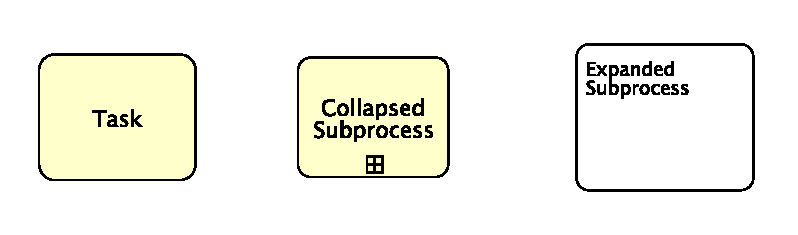
\includegraphics[width=0.5\textwidth]{images/processes.pdf}
\caption{BPMN activities: task, collapsed process, expanded subprocess}
\label{fig:task}
\end{figure}

\emph{Gateways} serve as means to control the flow of sequence in the diagram. As the term already implies, a gateway needs some ``mechanism that either allows or disallows passage through'' \citep{White:2004}. The result of a gateway pass-through can be that processes are merged or split. Graphically, a gateway is represented as a diamond. 

\begin{figure}[h]
\centering
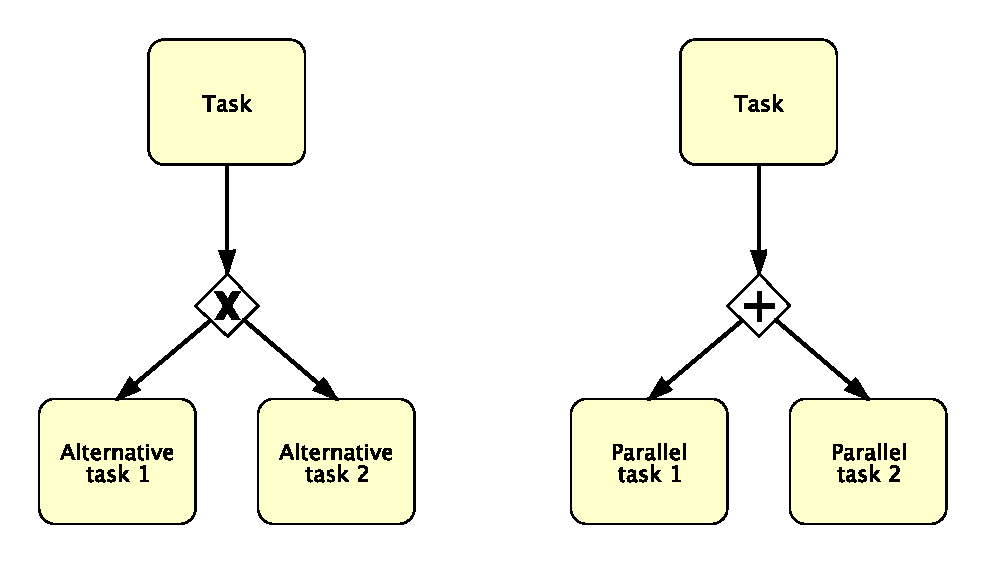
\includegraphics[width=0.5\textwidth]{images/gateways.pdf}
\caption{BPML gateway types: Exclusive (left), parallel (right)}
\label{fig:gateways}
\end{figure}

While there exist a number of different gateway types \citep[p.~93]{White:2004}, the SED-ML specification only uses the parallel and the exclusive gates  (\fig{gateways}). 

\emph{Exclusive} gateways -- also denoted as decisions -- allow the sequence flow to take two or more alternative paths (\fig{gateways}, left hand side). However, \emph{only one} of the paths may be chosen (not more). Sometimes two alternative branches need to be merged together again, in which case the exclusive gate must be used as well: The sequence flow continues as soon as \emph{one} of the incoming processes send a signal. An exclusive gateways is marked by an \code{X} in the graphical notation.

\emph{Parallel} gateways, ``provide a mechanism to synchronize parallel flow and to create parallel flow'' \citep{White:2004} (\fig{gateways}, right hand side). They are used to show parallel paths in the workflow; even if sometimes not required they might help in understanding the process. Synchronisation allows to start two processes in parallel at the same time in the sequence flow: The sequence flow will continue with \emph{all} processes leaving the parallel gateway. Joining two processes with a parallel gateway is also possible: the process flow will only continue after a signal has arrived from \emph{all} processes coming in the parallel gateway. A parallel gateway is marked by a \code{+} in the graphical notation.

\emph{Events} mark everything happening during the execution of the sequence flow, usually they interrrupt the business process, having some cause or impact on the execution. From the broad range of events that BPMN offers, SED-ML only uses a small subset, namely the start event and the end event (\fig{connectorEvents}).

\begin{figure}[h]
\centering
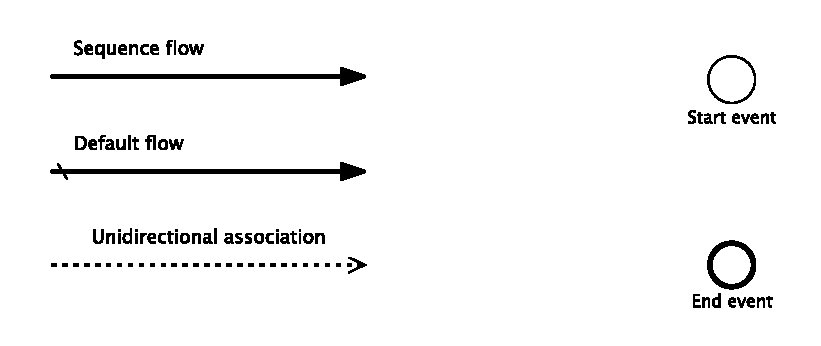
\includegraphics[width=0.5\textwidth]{images/connectors.pdf}
\caption{BPML connectors (left) and events (right).}
\label{fig:connectorEvents}
\end{figure}

All events are graphically drawn as small circles. A \emph{start event} is drawn with a single thin line and mark the start of a process, it can not have any incoming sequence flow. Start events may be triggered by different mechanisms, for the case of SED-ML the untyped start event (no marker inside the circle) is used. The trigger to start the process is ``Create new simulation experiment''. The \emph{end event} is marked with a thick line. It indicates the end of a process. SED-ML specification makes use of the untyped end event (no marker inside the circle). The end event is used to show the end of sub-processes as well as processes. If the end of a sub-process is reached, the sequence flow returns to the according parent process.

\emph{Connectors} are used to combine different BPMN objects with each other (\citet[p.~30]{White:2004} show the full list of valid connections). SED-ML uses only a subset of available connectors, namely sequence flow, default flow, and unidirectional associations (\fig{connectorEvents}). \emph{Sequence flow} defines the execution order of activities. \emph{Default flow} marks the default branch to be chosen if other conditions leave various possibilities for further execution of the sequence flow. A \emph{unidirectional association} is used to indicate that a data object is modified, i.\,e. read and written during the execution of an activity \citep{bpmnPoster}.

%
The rough SED-ML workflow is shown in Figure \ref{fig:sedmlWorkflow}.
%
\begin{figure}[h]
\centering
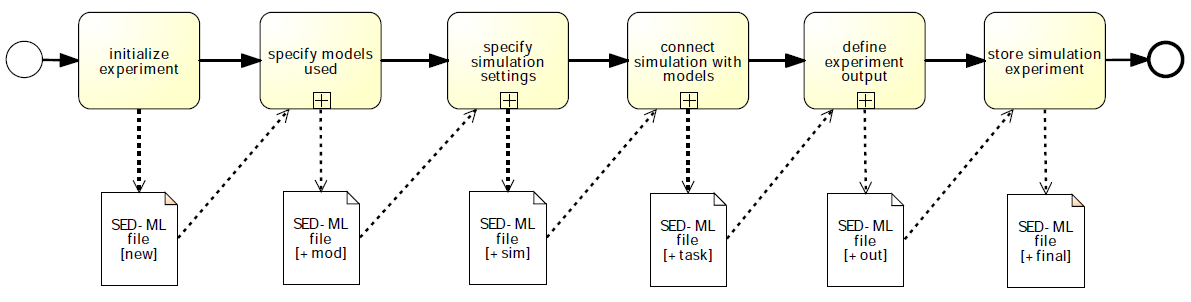
\includegraphics[width=\textwidth]{images/bpmn/sedMainOryx.png}
\caption{The process of defining a simulation experiment in SED-ML (overview)}
\label{fig:sedmlWorkflow}
\end{figure}
%
The process of defining a SED-ML simulation experiment starts by initialising the experiment and creating a new SED-ML file. Afterwards, the \concept{models} needed for the simulation are specified and stored into the existing SED-ML file (Section~\ref{overview:models}). In a third step, the simulation experiment \concept{setups} are defined and stored into the same file (Section~\ref{overview:simulation}). To assign a setup to a number of models used in the experiment, these connections have to be defined and recorded (Section~\ref{overview:task}), called \concept{task} in SED-ML. After simulation, the \concept{output} should be defined, based on the specified tasks and performed simulation experiment. The information is added to the existing SED-ML file (Section~\ref{overview:output}). In the end, the whole experiment is stored in the final SED-ML file.
%
All collapsed processes are described in the following sections. Examples in XML are provided in the more technical description.

\subsection{Models}
\label{overview:models}
To define a simulation experiment, first of all a new SED-ML file is created. The models to be used in the experiment (zero or many) are referenced, using a link to a model description in some open, curated model database (e.\,g.\ Biomodels Database \citep{LDR+10} or CellML Repository \citep{BBC+09}). All necessary changes to correctly simulate the model are defined, e.\,g., assigning new parameter values or updating the mathematics of the model (Figure~\ref{fig:workflowModel}).
%
\begin{figure}[h]
\centering
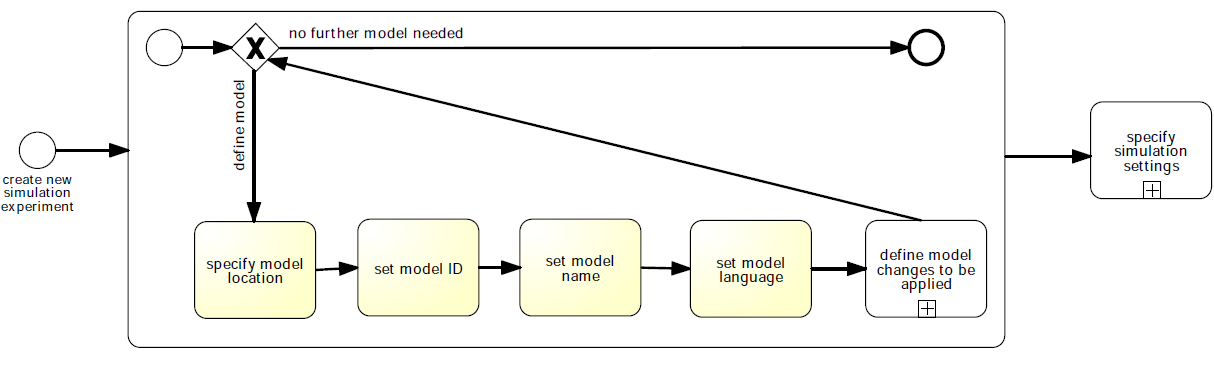
\includegraphics[width=0.8\textwidth]{images/bpmn/sedModelOryx.png}
\caption{The process of defining model(s) in SED-ML}
\label{fig:workflowModel}
\end{figure}
%
The procedure is repeated until all models participating in the experiment have been described. Each such model gets an internal SED-ML ID and an optional name.

\subsection{Simulation setup}
\label{overview:simulation}
Secondly, the simulation setups (zero or many) used throughout the simulation experiment are described (Figure \ref{fig:workflowSimulation}). 
%
%
\begin{figure}[h]
\centering
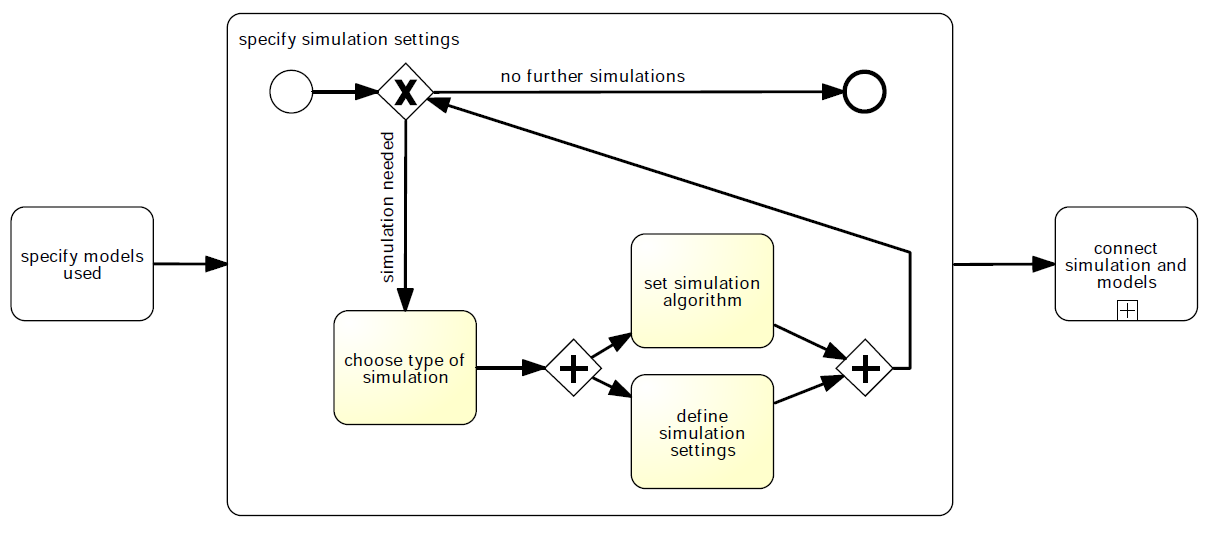
\includegraphics[width=0.8\textwidth]{images/bpmn/sedSimulationOryx.png}
\caption{The process of defining simulation(s) in SED-ML}
\label{fig:workflowSimulation}
\end{figure}
%
Those may stem from various different types of simulation, e.\,g., steady state analysis or bifurcation.  Depending on the specific type of experiment, the information encoded for the simulation setup might differ. Thus, the definition of simulation settings is specific to the simulation experiment.

In a simple case the experiment consists of one simulation, but it can get far more complex. For example, one might define a nested sequence of simulations, in which case every simulation has to be defined separately.
Each simulation setup gets its own internal ID and an optional name. For each of the setups, the simulation algorithm to be used for that simulation is defined through a reference to a well-defined algorithm name, e.\,g. an ontology or controlled vocabulary. One approach to define such a controlled vocabulary of simulation algorihtms is the \emph{Kinetic Simulation Algorithm Ontology} (Section~\ref{sec:kisao}). 
%
The setup definition is repeated until all different simulations have been described.

\subsection{Task}
\label{overview:task}
SED-ML allows to apply one defined simulation setting to one defined model at a time. However, any number of \concept{tasks} may be defined inside a simulation experiment description (Figure \ref{fig:workflowTask}). 
%
\begin{figure}[h]
\centering
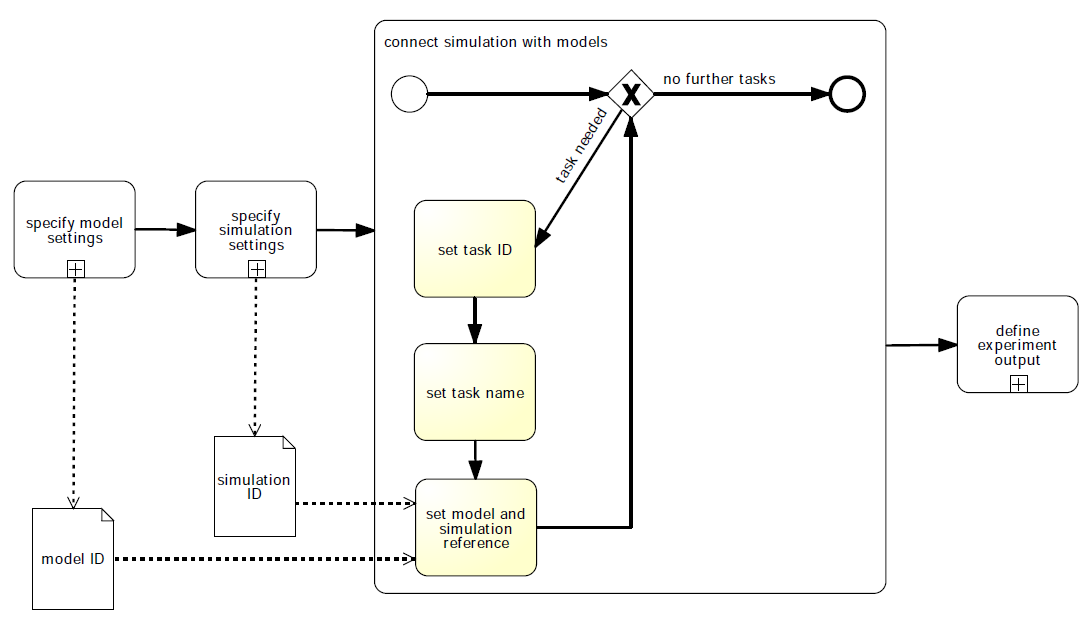
\includegraphics[width=0.7\textwidth]{images/bpmn/sedTaskOryx.png}
\caption{The process of defining simulation task(s) in SED-ML}
\label{fig:workflowTask}
\end{figure}
%
To do so, each task refers to one of the formerly specified models and to one of the formerly specified simulation setups. Each task has its own ID and an optional name. The process of task definition is repeated until all tasks have been defined.


The current SED-ML does not allow to nest or order tasks. However, these features are evaluated for future versions of SED-ML.

\subsection{Output}
\label{overview:output}
The SED-ML finally consists of output definitions that describe what kind of output the experiment uses to present the simulation result to the user, i.\,e., a plot or a data table (Figure \ref{fig:workflowOutput}), and also which data is part of the output. 
%
\begin{figure}[h]
\centering
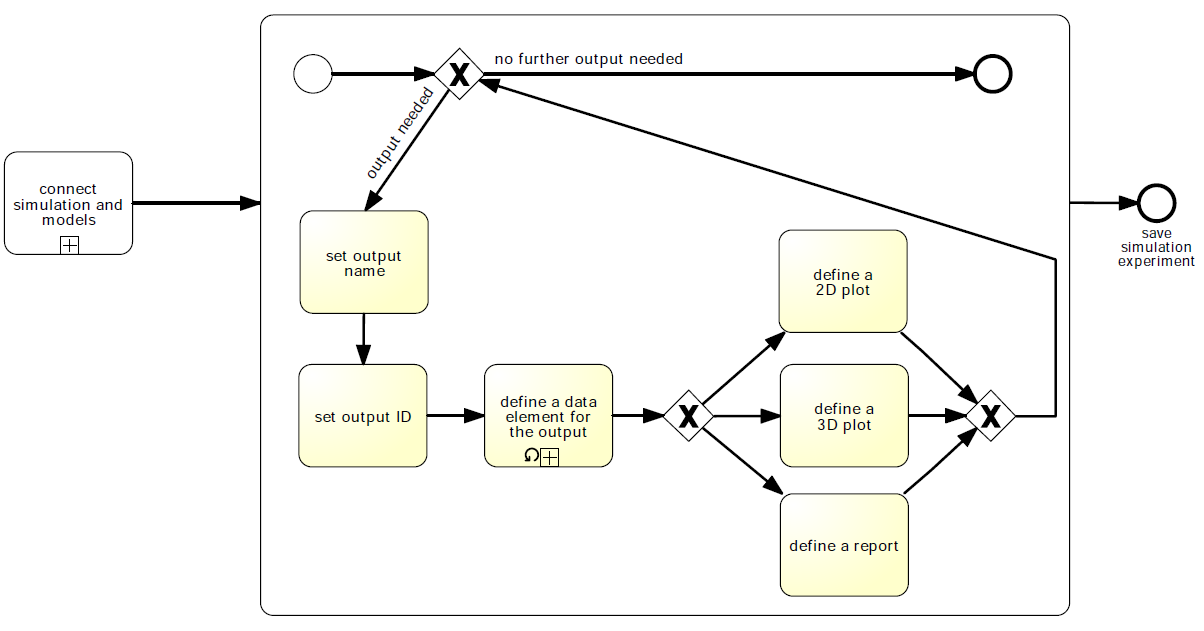
\includegraphics[width=0.7\textwidth]{images/bpmn/sedOutputOryx.png}
\caption{The process of defining output(s) in SED-ML}
\label{fig:workflowOutput}
\end{figure}
%
Therefore, SED-ML first defines a set of \concept{data generators} (Figure \ref{fig:workflowDataGenerator}), which are then used to specify a particular result, i.\,e. output (Section~\ref{overview:dataGen}). 

The SED-ML specification comes with three pre-defined types of outputs: 2D- and 3D plots, and reports. All use the aforementioned data generators to specify the information to be plotted on the different axes, or in the table comlumns respectively.
\subsection{Data Generator}
\label{overview:dataGen}
%
\begin{figure}[h]
\centering
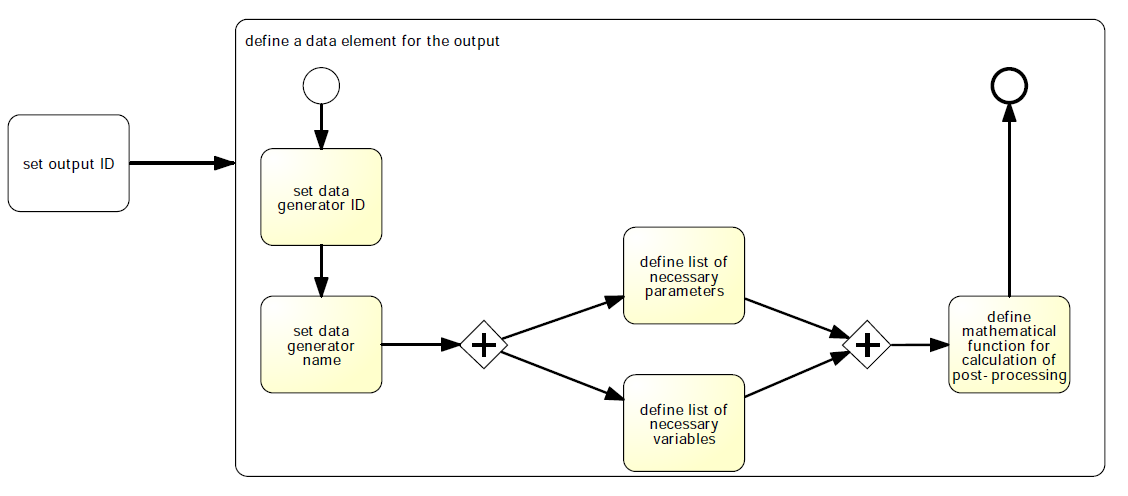
\includegraphics[width=0.7\textwidth]{images/bpmn/sedDataGeneratorOryx.png}
\caption{The process of defining data generator(s) in SED-ML}
\label{fig:workflowDataGenerator}
\end{figure}
%
A data generator may use data elements, e.\,g., variables or parameters, that either (1) have been taken directly from the model, or (2) have been generated in a post-processing step. If post-processing needs to be applied, variables and parameters from the various, previously defined models may be used, but also existing global parameters, such as \emph{time}.
If the variables are taken from existing models, a reference to the model and the particular variable needs to be given. 
If post-processing is necessary, a reference to an existing variable or parameter, including other data generators, has to be provided. Additional mathematical rules to be applied on the referred variable or parameter must then  be specified. 
%
In a SED-ML file, any number of data generators can be created for later re-use in the output definition.



%%% Local Variables: 
%%% mode: latex
%%% TeX-master: "../sed-ml-L1V2"
%%% End: 
